\section{KIẾN TRÚC HỆ THỐNG}
\begin{figure}[h]
    \centering
    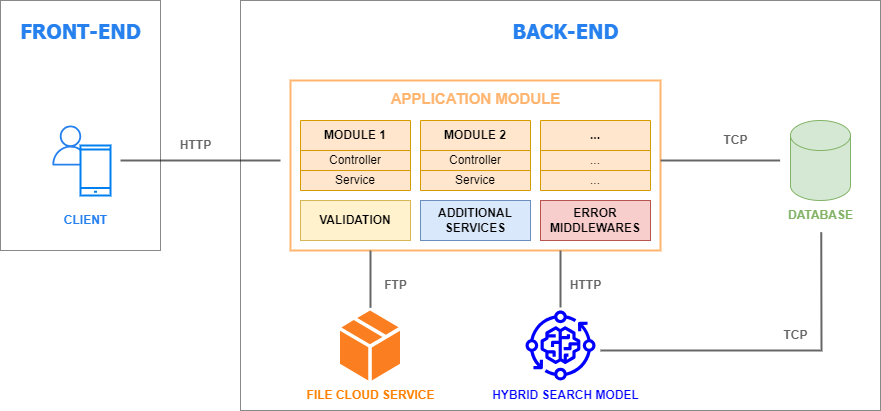
\includegraphics[width=1\textwidth]{Images/SystemArchitecture.png}
    \caption{Sơ đồ kiến trúc của ứng dụng Housernet}
\end{figure}
Ứng dụng Housernet sẽ được chia ra làm hai phần độc lập với nhau là \textit{front-end} và \textit{back-end}, trong đó phía \textit{client} sẽ gọi đến các chức năng của \textit{server} thông qua giao thức \textit{HTTP}, và phía \textit{server} sẽ được tổ chức thành các thành phần cụ thể khác nhau để xử lý cho các chức năng khác nhau. Một cách cụ thể hơn, kiến trúc này sẽ được chia ra thành các phần chính bao gồm:
\begin{itemize}
    \item \textit{Application module:} Đây là thành phần chính của \textit{back-end}, chứa đựng toàn bộ các chức năng nghiệp vụ của ứng dụng. Thành phần này sẽ chịu trách nhiệm chính trong việc giao tiếp với phía \textit{front-end} cho các yêu cầu xử lý từ phía người dùng. Mỗi chức năng sẽ được tổ chức thành mỗi \textit{module}, trong mỗi \textit{module} sẽ bao gồm \textit{controller} để tiếp nhận yêu cầu từ phía \textit{client} và thực hiện gọi phương thức phù hợp với yêu cầu nghiệp vụ ở tầng \textit{service}, như thế thành phần \textit{service} là nơi chứa đựng xử lý \textit{logic} chính cho chức năng đó. Bên cạnh đó, \textit{application module} còn có các thành phần xử lý khác bao gồm \textit{validation} - chịu trách nhiệm để kiểm tra tính hợp lệ của các yêu cầu gửi lên từ phía \textit{client}, \textit{additional services} - nơi tích hợp các chức năng từ bên thứ ba, bao gồm dịch vụ để kết nối với cơ sở dữ liệu thông qua \textit{ORM}, dịch vụ lưu trữ \textit{file} đám mây, dịch vụ \textit{vector embedding} cho văn bản, và cuối cùng là thành phần \textit{error middlewares} - chịu trách nhiệm bắt các lỗi liên quan đến thao tác với cơ sở dữ liệu.
    \item \textit{File cloud service:} Đây là nơi cung cấp dịch vụ lưu trữ \textit{file} đám mây, dịch vụ này được kết nối với \textit{application module} thông qua giao thức \textit{FTP}. Dịch vụ này được sử dụng cho mục đích tải \textit{file} do người dùng tải lên và lưu trữ, sau đó dịch vụ này sẽ trả về địa chỉ \textit{URL} để người dùng có thể truy cập trực tiếp vào \textit{file} tương ứng.
    \item \textit{Hybrid search model:} Thành phần này cung cấp chức năng tìm kiếm kết hợp, được xem như là tính năng chính cho ứng dụng. Thành phần này được triển khai tách biệt hoàn toàn so với \textit{application module} và sẽ cung cấp \textit{API} để cho \textit{application module} có thể gọi tới khi có yêu cầu liên quan đến chức năng tìm kiếm kết hợp. Ngoài ra thành phần này cũng giao tiếp với cơ sở dữ liệu bằng giao thức \textit{TCP} để có thể truy vấn kết quả tìm kiếm từ cơ sở dữ liệu ứng với yêu cầu đầu vào của người dùng.
    \item \textit{Database:} Thành phần này là nơi để triển khai cơ sở dữ liệu cho toàn bộ chức năng của ứng dụng, thành phần này có thể giao tiếp với thành phần \textit{application module} và thành phần \textit{hybrid search model} thông qua giao thức \textit{TCP}. Để có thể thực hiện chức năng tìm kiếm ngữ nghĩa, cơ sở dữ liệu phải có khả năng tích hợp \textit{vector database extension}. Nhờ đó mà cơ sở dữ liệu có khả năng lưu trữ dữ liệu ở kiểu \textit{vector} cũng như cho phép các truy vấn dựa trên \textit{vector}.
\end{itemize}